\documentclass[11pt,letterpaper]{article}
\usepackage[utf8]{inputenc}
\usepackage{amsmath,amssymb,fullpage,graphicx}

\begin{document}
\subsection*{Lect 9-1}
\noindent Given the model $Y_{ij} = \mu_i \epsilon_{ij}$ where $\epsilon \sim N(0, \sigma_{\epsilon})$. Then $Y_{ij} \sim N(\mu_i, \sigma_{\epsilon})$ \\

The likelihood function of data $Y_{ij}$'s is written as 
\begin{align*}
L(\mu_i, \sigma_{\epsilon} | Y) &= \prod_i^a \prod_j^n \text{pdf of Y} \\
&= \prod_i^a \prod_j^n \frac{1}{\sqrt{2 \pi \sigma^2}} e^{-\frac{1}{2} (\frac{Y_{ij} - \mu_i}{\sigma_{\epsilon}})^2} \\
&= e^{-\frac{1}{2} \sum_i^a \sum_j^n (\frac{Y_{ij} - \mu_i}{\sigma})^2 - \frac{1}{2} log(2 \pi \sigma^2)} \\
\end{align*}
\noindent To find the maximum point of likelihood function, find minimum value of exponent $-\frac{1}{2} \sum_i^a \sum_j^n (\frac{Y_{ij} - \mu_i}{\sigma})^2 - \frac{1}{2} log(2 \pi \sigma^2)$  
\begin{align*}
\frac{\partial exponent}{\partial \mu_i} &= \partial -\frac{1}{2} \sum_i^a \sum_j^n (\frac{Y_{ij} - \mu_i}{\sigma})^2 - \frac{1}{2} log(2 \pi \sigma^2) / \partial \mu_i \\
&= -\frac{1}{2} \sum_i^a \sum_j^n \partial (\frac{Y_{ij} - \mu_i}{\sigma})^2 / \partial \mu_i
\end{align*}
Note that $\mu_k$ only counts for $k$th level, therefore, 
\begin{align*}
\frac{1}{2} \sum_i^a \sum_j^n \partial (\frac{Y_{ij} - \mu_i}{\sigma})^2 / \partial \mu_k &= -\frac{1}{2} \sum_j^n \partial (\frac{Y_{kj} - \mu_k}{\sigma})^2 / \partial \mu_k \\
&= \frac{1}{\sigma^2} \sum_j^n (Y_{kj} - \mu_k)
\end{align*}
\begin{align*}
\frac{\partial exponent}{\partial \sigma_{\epsilon}} &= \partial -\frac{1}{2} \sum_i^a \sum_j^n (\frac{Y_{ij} - \mu_i}{\sigma})^2 - \frac{1}{2} log(2 \pi \sigma^2) / \partial \sigma_{\epsilon} \\
&= \frac{1}{\sigma^3} \sum_i^a \sum_j^n (Y_{ij} - \mu_i)^2 - \frac{N}{\sigma}
\end{align*}
\noindent Let $\frac{\partial L}{\partial \mu_i} = 0$ and $\frac{\partial L}{\partial \sigma_{\epsilon}}  = 0$
\begin{align*}
\frac{1}{\sigma^2} \sum_j^n (Y_{kj} - \mu_k) &= 0 \\
\sum_j^n (Y_{kj} - \mu_k)  &= 0 \\
Y_{i.} - n \hat{\mu_i} &= 0 \\
\hat{\mu_i} &= \bar{Y_{i.}}
\end{align*}
\begin{align*}
\frac{1}{\sigma^3} \sum_i^a \sum_j^n (Y_{ij} - \mu_i)^2 - \frac{N}{\sigma} &= 0 \\
\sigma_{\epsilon}^2 &= \frac{1}{N} \sum_i^a \sum_j^n (Y_{ij} - \hat{\mu_i})^2 \\
\end{align*}
\noindent Plug in the estimator of $ \mu_i$ as $\bar{Y_{i.}}$
\begin{align*}
\hat{\sigma_{\epsilon}} &=  \frac{1}{N} \sum_i^a \sum_j^n (Y_{ij} - \bar{Y_{i.}} )^2 \\
&= \frac{SSE}{N} \approx \frac{SSE}{N-a} = MSE
\end{align*}
\noindent The most likelihood estimator $\hat{\mu_i} = \bar{Y_{i.}}$, $\hat{\sigma_{\epsilon}} = \frac{SSE}{N}$

\subsection*{Lect 9-2}
\subsection*{a}
\noindent From the partial derivative on $\mu$ and $\tau_i$, we get equations 
\begin{align*}
Y_{..} - N \hat{\mu} - n\hat{\tau_.} &= 0 \\
Y_{i.} - n \hat{\mu} - n\hat{\tau_i} &= 0
\end{align*}
\noindent Plug in the constraint $\hat{\tau_.} = 0$ to equation one
\begin{align*}
Y_{..} - N \hat{\mu} &= 0 \\
\hat{\mu} &= \bar{Y_{..}}
\end{align*}
\noindent Plug in the estimator for $\mu$ to equations $Y_{i.} - n \hat{\mu} - n\hat{\tau_i} = 0$
\begin{align*}
Y_{i.} - n\bar{Y_{..}} - n\hat{\tau_i} &= 0 \\
\hat{\tau_i} &= \bar{Y_{i.}} - \bar{Y_{..}}
\end{align*}
\begin{align*}
\hat{Y_{ij}} = \hat{\mu} + \hat{\tau_i} =  \bar{Y_{..}} + \bar{Y_{i.}} - \bar{Y_{..}} = \bar{Y_{i.}}
\end{align*}

\subsection*{b}
\noindent Use any constraint $\hat{\tau_k} = c$ where c is a constant, $k \in 1, 2, ... a$. Plug in this constraint to equation $Y_{k.} - n \hat{\mu} - n \hat{\tau_k} = 0$
\begin{align*}
Y_{k.}  - n \hat{\mu} &= c \\
\hat{\mu} &= \bar{Y_{k.}} - \frac{c}{n}
\end{align*}
\noindent Plug in the constraint $\hat{\mu} = \bar{Y_{k.}} - \frac{c}{n}$ in to equation $Y_{i.} - n \hat{\mu} - n\hat{\tau_i} = 0$ for $i \neq k$
\begin{align*}
Y_{i.} - n \bar{Y_{k.}} + c - n \hat{\tau_i} &= 0 \\
\tau_i &= \bar{Y_{i.}} - \bar{Y_{k.}} + \frac{c}{n}
\end{align*}
\begin{align*}
Y_{ij} &= \hat{\mu} + \hat{\tau_i} = \bar{Y_{k.}} - \frac{c}{n} + \bar{Y_{i.}} - \bar{Y_{k.}} + \frac{c}{n} = \bar{Y_{i.}} 
\end{align*}

\noindent Therefore, in general, constraint doesn't change prediction $Y_{ij}$. 

\subsection*{Lect 9-3}
\subsection*{a}
\noindent From the partial derivative on $\mu$ and $\tau_i$, we get equations 
\begin{align*}
Y_{..} - N \hat{\mu} - n\hat{\tau_.} &= 0 \\
Y_{i.} - n \hat{\mu} - n\hat{\tau_i} &= 0
\end{align*}
\noindent Plug in the constraint $\hat{\tau_.} = 0$ to equation one
\begin{align*}
Y_{..} - N \hat{\mu} &= 0 \\
\hat{\mu} &= \bar{Y_{..}}
\end{align*}
\noindent Plug in the estimator for $\mu$ to equations $Y_{i.} - n \hat{\mu} - n\hat{\tau_i} = 0$
\begin{align*}
Y_{i.} - n\bar{Y_{..}} - n\hat{\tau_i} &= 0 \\
\hat{\tau_i} &= \bar{Y_{i.}} - \bar{Y_{..}}
\end{align*}

\subsection*{b}
\noindent From part a, we have known that estimator for $\tau_i$ is $\bar{Y_{i.}} - \bar{Y_{..}}$, then $\hat{\tau_1} = \bar{Y_{1.}} - \bar{Y_{..}}$, $\hat{\tau_2} = \bar{Y_{2.}} - \bar{Y_{..}}$, $\hat{\tau_3} = \bar{Y_{3.}} - \bar{Y_{..}}$
\begin{align*}
\hat{\tau_1} - \hat{\tau_2} &= \bar{Y_{1.}} - \bar{Y_{..}} - \bar{Y_{2.}} + \bar{Y_{..}} = \bar{Y_{1.}} - \bar{Y_{2.}} \\
\hat{\tau_1} - \hat{\tau_3} &= \bar{Y_{1.}} - \bar{Y_{..}} - \bar{Y_{3.}} + \bar{Y_{..}} = \bar{Y_{1.}} - \bar{Y_{3.}} \\
\hat{\tau_2} - \hat{\tau_3} &= \bar{Y_{2.}} - \bar{Y_{..}} - \bar{Y_{3.}} + \bar{Y_{..}} = \bar{Y_{2.}} - \bar{Y_{3.}} 
\end{align*}

\subsection*{c}
\noindent From the partial derivative on $\mu$ and $\tau_i$, we get equations 
\begin{align*}
Y_{..} - N \hat{\mu} - n\hat{\tau_.} &= 0 \\
Y_{i.} - n \hat{\mu} - n\hat{\tau_i} &= 0 \text{, i = 1,2,3 ... a}
\end{align*}
Plug in the constraint $\hat{\tau_3} = 0$ to equation $Y_{3.} - n \hat{\mu} - n\hat{\tau_3} = 0$
\begin{align*}
Y_{3.} - n \hat{\mu} &= 0 \\
\hat{\mu} &= \frac{Y_{3.}}{n} = \bar{Y_{3.}}
\end{align*}
Plug in the constraint $\hat{\mu} = \bar{Y_{3.}}$ to equations $Y_{i.} - n \hat{\mu} - n\hat{\tau_i} = 0$ for $i = 1,2,4... a$
\begin{align*}
Y_{i.} - n\bar{Y_{3.}} - n \hat{\tau_i} &= 0 \\
\tau_i &= \bar{Y_{i.}} - \bar{Y_{3.}}
\end{align*}

\subsection*{d}
\noindent From part c, we have known that estimator for $\tau_i$ is $\bar{Y_{i.}} - \bar{Y_{3.}}$, then $\hat{\tau_1} = \bar{Y_{1.}} - \bar{Y_{3.}}$, $\hat{\tau_2} = \bar{Y_{2.}} - \bar{Y_{3.}}$, $\hat{\tau_3} = 0$
\begin{align*}
\hat{\tau_1} - \hat{\tau_2} &= \bar{Y_{1.}} - \bar{Y_{3.}} - \bar{Y_{2.}} + \bar{Y_{3.}} = \bar{Y_{1.}} - \bar{Y_{2.}} \\
\hat{\tau_1} - \hat{\tau_3} &= \bar{Y_{1.}} - \bar{Y_{3.}} \\
\hat{\tau_2} - \hat{\tau_3} &= \bar{Y_{2.}} - \bar{Y_{3.}} 
\end{align*}

\subsection*{e}
\noindent estimator for $\mu + \tau_1$ with constraint in part a is 
\begin{align*}
\mu + \tau_1 &= \bar{Y_{..}} + \bar{Y_{1.}} - \bar{Y_{..}} = \bar{Y_{1.}} 
\end{align*}
\noindent estimator for $\mu + \tau_1$ with constraint in part c is 
\begin{align*}
\mu + \tau_1 &= \bar{Y_{3.}} + \bar{Y_{1.}} - \bar{Y_{3.}} = \bar{Y_{1.}} 
\end{align*}

\noindent estimator for $2 \tau_1 - \tau_2 - \tau_3$ with constraint in part a is 
\begin{align*}
2 \tau_1 - \tau_2 - \tau_3 &= 2 \bar{Y_{1.}} - 2\bar{Y_{..}} - \bar{Y_{2.}} + \bar{Y_{..}} - \bar{Y_{3.}} + \bar{Y_{..}} = 2 \bar{Y_1.} - \bar{Y_{2.}} - \bar{Y_{3.}}
\end{align*}
\noindent estimator for $2 \tau_1 - \tau_2 - \tau_3$ with constraint in part c is 
\begin{align*}
2 \tau_1 - \tau_2 - \tau_3 &= 2 \bar{Y_{1.}} - 2\bar{Y_{3.}} - \bar{Y_{2.}} + \bar{Y_{3.}} = 2 \bar{Y_1.} - \bar{Y_{2.}} - \bar{Y_{3.}}
\end{align*}

\noindent estimator for $\mu + \tau_1 + \tau_2$ with constraint in part a is 
\begin{align*}
\mu + \tau_1 + \tau_2 &= \bar{Y_{..}} + \bar{Y_{1.}} - \bar{Y_{..}} + \bar{Y_{2.}} - \bar{Y_{..}} = \bar{Y_{1.}} + \bar{Y_{2.}} - \bar{Y_{..}}
\end{align*}
\noindent estimator for $\mu + \tau_1 + \tau_2$ with constraint in part c is 
\begin{align*}
\mu + \tau_1 + \tau_2 &= \bar{Y_{3.}} + \bar{Y_{1.}} - \bar{Y_{3.}} + \bar{Y_{2.}} - \bar{Y_{3.}} = \bar{Y_{1.}} + \bar{Y_{2.}} - \bar{Y_{3.}}
\end{align*}

\noindent First and second contrasts do not depend on the constraint, implying first and second contrasts are estimable. 

\subsection*{Lect 10-1}
\subsection*{a}
\noindent $Y_{ij} \sim N(\mu, \sigma_{\epsilon})$
\begin{align*}
L(\mu, \sigma_{\epsilon} | Y) &= \prod_i^a \prod_j^n \text{pdf of Y} \\
&= \prod_i^a \prod_j^n \frac{1}{\sqrt{2 \pi \sigma^2}} e^{-\frac{1}{2} (\frac{Y_{ij} - \mu}{\sigma_{\epsilon}})^2} \\
&= e^{-\frac{1}{2} \sum_i^a \sum_j^n (\frac{Y_{ij} - \mu}{\sigma})^2 - \frac{1}{2} log(2 \pi \sigma^2)} \\
\end{align*}
\noindent To find the maximum point of likelihood function, find minimum value of exponent $-\frac{1}{2} \sum_i^a \sum_j^n (\frac{Y_{ij} - \mu}{\sigma})^2 - \frac{1}{2} log(2 \pi \sigma^2)$  
\begin{align*}
\frac{\partial exponent}{\partial \mu} &= \partial -\frac{1}{2} \sum_i^a \sum_j^n (\frac{Y_{ij} - \mu}{\sigma})^2 - \frac{1}{2} log(2 \pi \sigma^2) / \partial \mu_i \\
&= -\frac{1}{2} \sum_i^a \sum_j^n \partial (\frac{Y_{ij} - \mu}{\sigma})^2 / \partial \mu_i \\
&= \sum_i^a \sum_j^n \frac{Y_{ij} - \mu}{\sigma^2} \\
&= (\sum_i^a \sum_j^n Yij - N \cdot \mu ) / \sigma^2
\end{align*}
\begin{align*}
\frac{\partial exponent}{\partial \sigma_{\epsilon}} &= \partial -\frac{1}{2} \sum_i^a \sum_j^n (\frac{Y_{ij} - \mu}{\sigma})^2 - \frac{1}{2} log(2 \pi \sigma^2) / \partial \sigma_{\epsilon} \\
&= \frac{1}{\sigma^3} \sum_i^a \sum_j^n (Y_{ij} - \mu)^2 - \frac{N}{\sigma}
\end{align*}
\noindent Let $\frac{\partial L}{\partial \mu} = 0$ and $\frac{\partial L}{\partial \sigma_{\epsilon}}  = 0$
\begin{align*}
(\sum_i^a \sum_j^n Yij - N \cdot \hat{\mu} ) / \sigma^2 &= 0 \\
\sum_i^a \sum_j^n Yij - N \cdot \hat{\mu} &= 0 \\
\hat{\mu} &= Y_{..} / N = \bar{Y_{..}}
\end{align*}
\noindent Plug in the estimator of $ \mu$ as $\bar{Y_{..}}$
\begin{align*}
\hat{\sigma_{\epsilon}} &=  \frac{1}{N} \sum_i^a \sum_j^n (Y_{ij} - \bar{Y_{..}} )^2 \\
&= \frac{SSE}{N} 
\end{align*}
\noindent The most likelihood estimator $\hat{\mu_i} = \bar{Y_{..}}$, $\hat{\sigma_{\epsilon}} = \frac{SSE}{N}$ \\

\noindent Using the estimator of $\mu$ and $\sigma_{\epsilon}$, $SSE(\mu) = \sum_i^a \sum_j^n (Y_{ij} - \hat{\mu})^2$ or $N \cdot \hat{\sigma}^2$

\subsection*{b}
\noindent Know that $\hat{\mu} = \bar{Y_{..}}$, $\hat{\tau_i} = \bar{Y_{i.}} - \bar{Y_{..}}$
\begin{align*}
SSE_{\mu, \tau_i} &= \sum_i^a \sum_j^n (Y_{ij} - \hat{\mu} - \hat{\tau_i})^2 \\
&= \sum_i^a \sum_j^n (Y_{ij} - \bar{Y_{..}} - \bar{Y_{i.}} + \bar{Y_{..}})^2 \\
&= \sum_i^a \sum_j^n (Y_{ij} - \bar{Y_{i.}})^2 \\
&= \sum_i^a \sum_j^n (Y_{ij} - \hat{\mu})^2 \\
&= N \cdot \hat{\sigma}^2
\end{align*}

\subsection*{c}
\begin{align*}
SSE(\mu) - SSE(\mu, \tau) &= [\sum_i^a \sum_j^n (Y_{ij} - \bar{Y_{..}})^2 ]- [\sum_i^a \sum_j^n (Y_{ij} - Y_{i.})^2] \\
&= \sum_i^a \sum_j^n [(Y_{ij} - \bar{Y_{..}})^2 - (Y_{ij} - \bar{Y_{i.}})^2] \\
&= \sum_i^a \sum_j^n [(Y_{ij} - \bar{Y_{..}}  + Y_{ij} - \bar{Y_{i.}} ) (Y_{ij} - \bar{Y_{..}} - Y_{ij} + \bar{Y_{i.}})] \\
&= \sum_i^a \sum_j^n [(2 Y_{ij} - \bar{Y_{..}}  - \bar{Y_{i.}} ) (\bar{Y_{i.}} - \bar{Y_{..}})] \\
&= \sum_i^a [\sum_j^n (2 Y_{ij} - \bar{Y_{..}}  - \bar{Y_{i.}} ) ] (\bar{Y_{i.}} - \bar{Y_{..}}) \\
&= \sum_i^a [(2 Y_{i.} - n\bar{Y_{..}}  - Y_{i.}) ] (\bar{Y_{i.}} - \bar{Y_{..}})\\
&= \sum_i^a n(\bar{Y_{i.}} - \bar{Y_{..}}) (\bar{Y_{i.}} - \bar{Y_{..}})\\
&= n \sum_i^a (\bar{Y_{i.}} - \bar{Y_{..}})^2 = SStr
\end{align*}
\noindent Then $F = \frac{MStr}{MSE} = \frac{SS_{treat}/ (a-1)}{SSE(\mu, \tau_i) / (N-a)} = \frac{SSE(\mu) - SSE(\mu, \tau_i) / (a-1)}{SSE(\mu, \tau_i) / (N-a)}$ 

\subsection*{Lect 10-2}
\begin{align*}
E(MS_{treat}) &= E(\frac{b \sum_i^a (\bar{Y_{i.}} - \bar{Y_{..}})^2}{a-1}) \\
&= \frac{b}{a-1} \sum_i^a E((\bar{Y_{i.}} - \bar{Y_{..}})^2) \\
&= \frac{b}{a-1} \sum_i^a E((\frac{\sum_j^b Y_{ij}}{b} - \frac{\sum_i^a \sum_j^b Y_{ij}}{ab})^2) \\
&= \frac{b}{a-1} \sum_i^a E((\frac{\sum_j^b \mu + \alpha_i + \beta_j + \epsilon_{ij}}{b} - \frac{\sum_i^a \sum_j^b \mu + \alpha_i + \beta_j + \epsilon_{ij}}{ab})^2) \\
&= \frac{b}{a-1} \sum_i^a E((\frac{\sum_j^b \mu + \alpha_i + \beta_j + \epsilon_{ij}}{b} - \frac{\sum_i^a \sum_j^b \mu + \alpha_i + \beta_j + \epsilon_{ij}}{ab})^2) \\
&= \frac{b}{a-1} \sum_i^a E((\frac{b \mu + b \alpha_i + \sum_j^b \beta_j + \epsilon_{ij}}{b} - \frac{ab \mu + \sum_i^a b \alpha_i + \sum_j^b a \beta_j +  \sum_i^a \sum_j^b \epsilon_{ij}}{ab})^2) \\
&= \frac{b}{a-1} \sum_i^a E((\mu + \alpha_i + \bar{\beta_.} + \bar{\epsilon_{i.}}  - \mu - \bar{\alpha_.}  - \bar{\beta_.} - \bar{\epsilon_{..}})^2) \\
&= \frac{b}{a-1} \sum_i^a  E((\alpha_i - \bar{\alpha_.}+ \bar{\epsilon_{i.}} - \bar{\epsilon_{..}}   )^2 )\\
&= \frac{b}{a-1} \sum_i^a  E((\alpha_i - \bar{\alpha_.})^2 + 2 (\alpha_i - \bar{\alpha_.})(\bar{\epsilon_{i.}} - \bar{\epsilon_{..}})  + (\bar{\epsilon_{i.}} - \bar{\epsilon_{..}})^2 ) \\
&= \frac{b}{a-1} \sum_i^a [E((\alpha_i - \bar{\alpha_.})^2) + E(2 (\alpha_i - \bar{\alpha_.})(\bar{\epsilon_{i.}} - \bar{\epsilon_{..}}) )  + E(\bar{\epsilon_{i.}} - \bar{\epsilon_{..}})^2) ]
\end{align*}
\noindent Note that $\alpha_i$'s are parameter $E( 2 (\alpha_i - \bar{\alpha_.})(\bar{\epsilon_{i.}} - \bar{\epsilon_{..}}) ) = 2(\alpha_i - \bar{\alpha_.}) E(\bar{\epsilon_{i.}} - \bar{\epsilon_{..}})$. Since $\epsilon_ij$ are iid's, $E(\bar{\epsilon_{i.}} - \bar{\epsilon_{..}}) = 0$, then $E( 2 (\alpha_i - \bar{\alpha_.})(\bar{\epsilon_{i.}} - \bar{\epsilon_{..}}) ) = 0$.
\begin{align*}
E(MS_{treat}) &= \frac{b}{a-1} \sum_i^a [E((\alpha_i - \bar{\alpha_.})^2) - \bar{\epsilon_{..}}) )  + E(\bar{\epsilon_{i.}} - \bar{\epsilon_{..}})^2) ] \\
&= \frac{b}{a-1} \sum_i^a [(\alpha_i - \bar{\alpha_.})^2 + \frac{1}{b} (1 - \frac{1}{a} \sigma^2)] \\
&= \frac{b}{a-1} \sum_i^a (\alpha_i - \bar{\alpha_.})^2 + \sigma_{\epsilon}^2
\end{align*}

\subsection*{Lect 10-3}
\subsection*{a}
\noindent Row means and variances $\bar{Y_{1.}} = \frac{4 + 6}{2} = 5$, $\bar{Y_{2.}} = \frac{10 + 2}{2} = 6$, $s_{1.}^2 = \frac{1}{2}(4-6)^2 = 2$, $s_{2.}^2 = \frac{1}{2} (10 - 2)^2 = 32$ \\

\noindent Col means and variances $\bar{Y_{.1}} = \frac{4 + 10}{2} = 7$, $\bar{Y_{.2}} = \frac{6 + 2}{2} = 4$, $s_{.1}^2 = \frac{1}{2}(4-10)^2 = 18$, $s_{.2}^2 = \frac{1}{2} (6 - 2)^2 = 8$ \\

\noindent $\bar{Y_{..}} = \frac{4 + 6 + 10 + 2}{4} = 5.5$, $SST = \sum_i^2 \sum_j^2 (Y_{ij} - \bar{Y_{..}})^2 = 35$

\subsection*{b}
\noindent For row quantities, variance of row means is $\frac{1}{2} ((5 - 5.5)^2 + (6 - 5.5)^2) = 0.25$. Sum of row variance is $2 + 32 = 34$. \\

\noindent $SStr = 2 \cdot $ variance of row means $= 0.5$, $SSE = $ sum of row variance $= 34$, $SST = n \cdot SStr + (n-1) \cdot SSE = 4 \cdot $ variance of row means $+ 2 \cdot $ sum of row variance $= 1 + 34 = 35 = SST$ 

\subsection*{c}
\noindent For row quantities, variance of col means is $\frac{1}{2} ((7 - 5.5)^2 + (4 - 5.5)^2) = 2.25$. Sum of col variance is $18 + 8 = 26$. \\

\noindent $SStr = 2 \cdot $ variance of col means $= 4.5$, $SSE = $ sum of col variance $= 26$, $SST = n \cdot SStr + (n-1) \cdot SSE = 4 \cdot $ variance of col means $+ 2 \cdot $ sum of col variance $= 9 + 26 = 35 = SST$ 

\subsection*{Lect 10-4}
\begin{verbatim}
b = 5
a = 4
data = matrix(0, ncol = b, nrow = a)
data[1,] = c(73, 68, 74, 71, 67)
data[2,] = c(73, 67, 75, 72, 70)
data[3,] = c(75, 68, 78, 73, 68)
data[4,] = c(73, 71, 75, 75, 69)
\end{verbatim}
\subsection*{a}
\begin{verbatim}
y <- as.vector(t(data))
A <- as.factor(rep(c(1:a), each=b))
B <- as.factor(rep(c(1:b), times=a))

SSE <- summary.aov(lm(y~A+B))[[1]]$`Sum Sq`[3]
F_block <- summary.aov(lm(y~A+B))[[1]]$`F value`[2]
F_treat <- summary.aov(lm(y~A+B))[[1]]$`F value`[1]


> SSE
[1] 21.8
> F_block
[1] 21.6055
> F_treat
[1] 2.376147
\end{verbatim}
\noindent SSE is 21.8, F-value for block factor is 21.6, F-value for treatment factor is 2.376

\subsection*{b}
\begin{verbatim}
lm1 <- summary.aov(lm(y~B))[[1]]
SSE1 <- lm1$`Sum Sq`[2]

> SSE1
[1] 34.75
\end{verbatim}
\noindent Exclude treatment factor, the SSE of reduced model is 34.75

\subsection*{c}
\begin{verbatim}
lm2 <- summary.aov(lm(y~A))[[1]]
SSE2 <- lm2$`Sum Sq`[2]

> SSE2
[1] 178.8
\end{verbatim}

\noindent Exclude block factor, the SSE of reduced model is 178.8

\subsection*{d}
\begin{align*}
F_{treat} = \frac{(SSE(\text{without treatment factor}) - SSE(\text{with treatment factor}) )  / (a - 1)}{SSE(\text{with treatment factor})  / (a - 1)(b - 1)}
\end{align*}
\begin{verbatim}
> ((SSE1 - SSE)/(a-1)) / (SSE/((a-1)*(b-1)))
[1] 2.376147
\end{verbatim}
\noindent This F ratio is equal to F ration of treatment factor in part a.

\begin{align*}
F_{block} = \frac{(SSE(\text{without block factor}) - SSE(\text{with block factor}) )  / (b - 1)}{SSE(\text{with block factor})  / (a - 1)(b - 1)}
\end{align*}
\begin{verbatim}
> ((SSE2 - SSE)/(b-1)) / (SSE/((a-1)*(b-1)))
[1] 21.6055
\end{verbatim}
\noindent This F ratio is equal to F ration of block factor in part a.

\subsection*{Lect 11-1}
\subsection*{a}
\begin{verbatim}
y <- as.vector(t(data))
grand_mean <- mean(y)
SSTr <- sum((apply(data, 1, mean) - grand_mean)^2) * b
SSE <- sum(apply(data, 1, var)) * (b-1)
F_ratio <- (SSTr / (a-1)) / (SSE / (a*b - a))
p_val <- pf(F_ratio, df1 = a-1, df2=a*b - a, lower.tail = F)

> p_val
[1] 0.764377
\end{verbatim}
\noindent By CRD model, under $H_0$ that treatment factor has no effect on strength, p-value of ANOVA one-way F-test is $0.76$, which is insignificant to reject null hypothesis. 

\subsection*{b}
\begin{verbatim}
A <- as.factor(rep(c(1:a), each=b))
B <- as.factor(rep(c(1:b), times=a))

yi. <- apply(data, 1, mean)
y.j <- apply(data, 2, mean)
SStr <- b * sum((yi. - grand_mean)^2)
SSbl <- a * sum((y.j - grand_mean)^2)
SST <- sum((y - grand_mean)^2)
SSE <- SST - SStr - SSbl
F_ratio <- (SStr / (a-1)) / (SSE / ((a-1)*(b-1)))
p_val <- pf(F_ratio, df1=a-1, df2=(a-1) * (b-1), lower.tail = F)

> p_val
[1] 0.1211445
\end{verbatim}
\noindent By RCBD model, under $H_0$ that treatment factor has no effect on strength, p-value of ANOVA one-way F-test is $0.121$, which is insignificant to reject null hypothesis. 

\subsection*{c}
\noindent In CRD, $\hat{Y_{ij}} = \hat{\mu} + \hat{\tau_i} = \bar{Y_{i.}}$
\begin{verbatim}
y_hat <- rep(yi., each=b)
resid <- y - y_hat
par(mfrow=c(1,2))
plot(x=y_hat, y=resid, xlab='Y-hat', ylab='Residuals')
abline(h=0, lty=2)
plot(x=y, y=resid, xlab='Y', ylab='Residuals')
\end{verbatim}
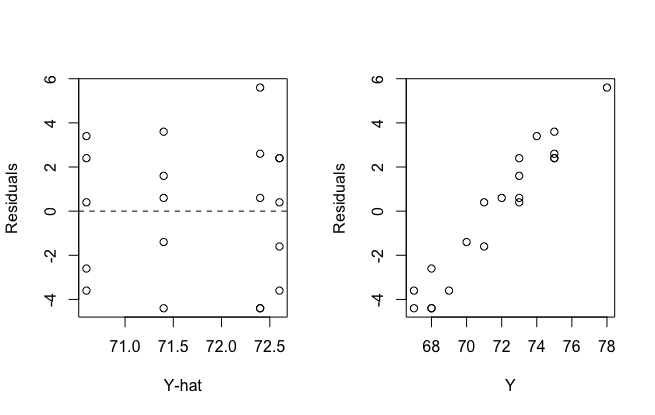
\includegraphics[scale=0.70]{lect-11-1-c.png}

\noindent The plot of residuals vs $\hat{Y}$ distributed randomly, implying the equal variance assumption is not violate. 

\subsection*{d}
\noindent In RCBD, $\hat{Y_{ij}} = \hat{\mu} + \hat{\alpha_i} + \hat{\beta_j} = \bar{Y_{i.}} + \bar{Y_{.j}} - \bar{Y_{..}}$ 
\begin{verbatim}
y_hat <- rep(yi., each=b) + rep(y.j, times=a) - grand_mean
resid <- y - y_hat
par(mfrow=c(1,2))
plot(x=y_hat, y=resid, xlab='Y-hat', ylab='Residuals')
abline(h=0, lty=2)
plot(x=y, y=resid, xlab='Y', ylab='Residuals')
\end{verbatim}
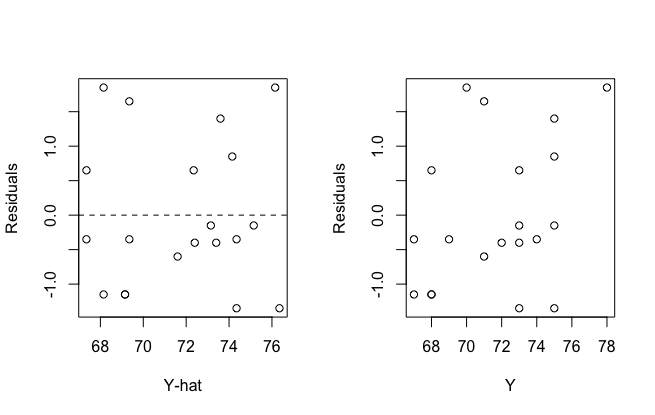
\includegraphics[scale=0.70]{lect-11-1-d.png}

\noindent The plot of residuals vs $\hat{Y}$ distributed randomly, implying the equal variance assumption is not violate. 


\subsection*{e}
\begin{verbatim}
y_hat1 <- rep(yi., each=b)
resid1 <- y - y_hat1
y_hat2 <- rep(yi., each=b) + rep(y.j, times=a) - grand_mean
resid2 <- y - y_hat2
par(mfrow=c(1,2))
qqnorm(resid1, main='CRD Residuals QQplot')
qqnorm(resid2, main='RCBD Residuals QQplot')
\end{verbatim}
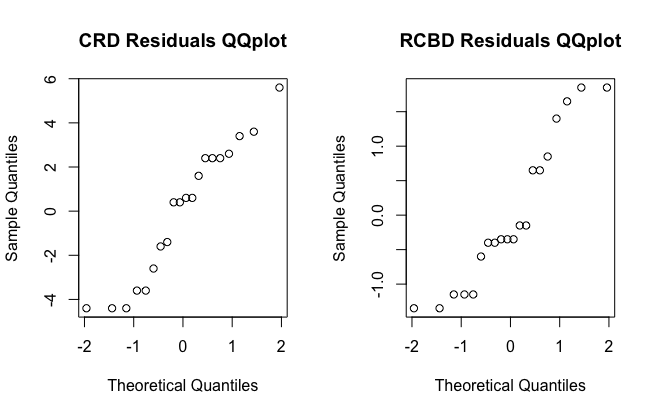
\includegraphics[scale=0.7]{lect-11-1-e.png}

\noindent The qqplots for both models have the shape of a line, implying the normality assumption is not violated. 

\subsection*{Lect 11-2}
\begin{tabular}{|ccc|}
\hline
A&B&C\\
\hline
B&C&A\\
\hline
C&A&B\\
\hline
\end{tabular}
\quad
\begin{tabular}{|ccc|}
\hline
A&B&C\\
\hline
C&A&B\\
\hline
B&C&A\\
\hline
\end{tabular}
\quad
\begin{tabular}{|ccc|}
\hline
A&C&B\\
\hline
B&A&C\\
\hline
C&B&A\\
\hline
\end{tabular}
\quad
\begin{tabular}{|ccc|}
\hline
A&C&B\\
\hline
C&B&A\\
\hline
B&A&C\\
\hline
\end{tabular}
\newline
\newline

\noindent \begin{tabular}{|ccc|}
\hline
B&A&C\\
\hline
A&C&B\\
\hline
C&B&A\\
\hline
\end{tabular}
\quad
\begin{tabular}{|ccc|}
\hline
B&A&C\\
\hline
C&B&A\\
\hline
A&C&B\\
\hline
\end{tabular}
\quad
\begin{tabular}{|ccc|}
\hline
B&C&A\\
\hline
A&B&C\\
\hline
C&A&B\\
\hline
\end{tabular}
\quad
\begin{tabular}{|ccc|}
\hline
B&C&A\\
\hline
C&A&B\\
\hline
A&B&C\\
\hline
\end{tabular}
\newline
\newline

\noindent \begin{tabular}{|ccc|}
\hline
C&A&B\\
\hline
A&B&C\\
\hline
B&C&A\\
\hline
\end{tabular}
\quad
\begin{tabular}{|ccc|}
\hline
C&B&A\\
\hline
A&C&B\\
\hline
B&A&C\\
\hline
\end{tabular}
\quad
\begin{tabular}{|ccc|}
\hline
C&B&A\\
\hline
B&A&C\\
\hline
A&C&B\\
\hline
\end{tabular}
\quad
\begin{tabular}{|ccc|}
\hline
C&A&B\\
\hline
B&C&A\\
\hline
A&B&C\\
\hline
\end{tabular}

\subsection*{Lect 11-3}
\noindent \begin{tabular}{|cccc|}
\hline
A&B&C&D\\
\hline
B&C&D&A \\
\hline
C&D&A&B\\
\hline
D&A&B&C\\
\hline
\end{tabular}
\quad
\begin{tabular}{|cccc|}
\hline
A&B&C&D\\
\hline
B&A&D&C \\
\hline
C&D&A&B\\
\hline
D&C&B&A\\
\hline
\end{tabular}
\quad
\begin{tabular}{|cccc|}
\hline
A&B&C&D\\
\hline
B&D&A&C \\
\hline
C&A&D&B\\
\hline
D&C&B&A\\
\hline
\end{tabular}
\quad
\begin{tabular}{|cccc|}
\hline
A&B&C&D\\
\hline
B&A&D&C \\
\hline
C&D&B&A\\
\hline
D&C&A&B\\
\hline
\end{tabular}



\end{document}